\documentclass[oneside,a4paper,12pt]{article}
\input preambulo.tex

\begin{document}
\maketitle
\FRASE

%\begin{figure}[h]
%\center
%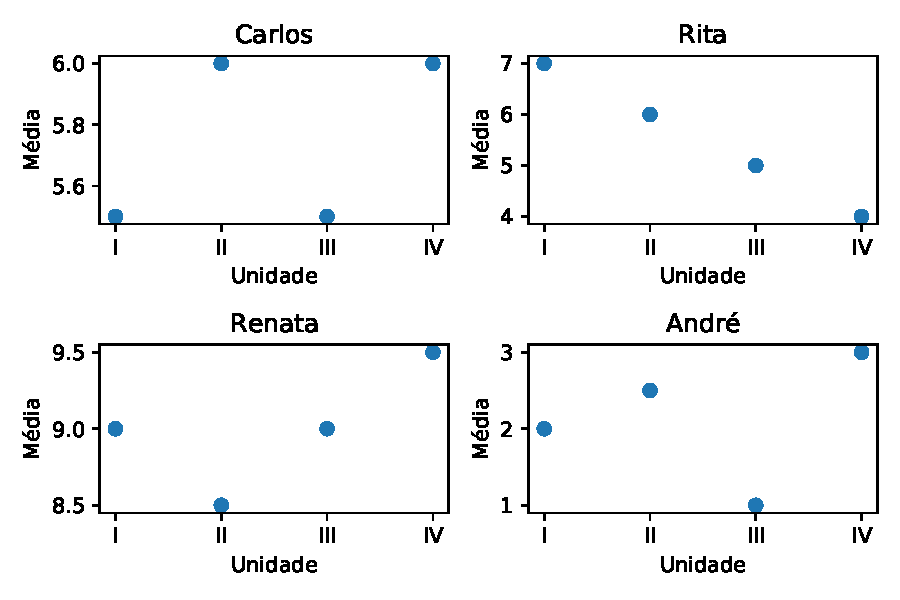
\includegraphics[width=5cm]{01}
%\end{figure}

\section*{A Fórmula de Euler}
A fórmula de Euler relaciona o número de vértices (\m{V}), faces (\m{F}) e arestas (\m{A}) de um poliedro convexo:

\M{V - A + F = 2} 

\subsection*{Problemas}
\begin{problema}
Complete as tabelas com o número de vértices arestas e faces dos poliedros a seguir:
\begin{figure}[!htb]
\begin{multicols}{2}
\begin{center}
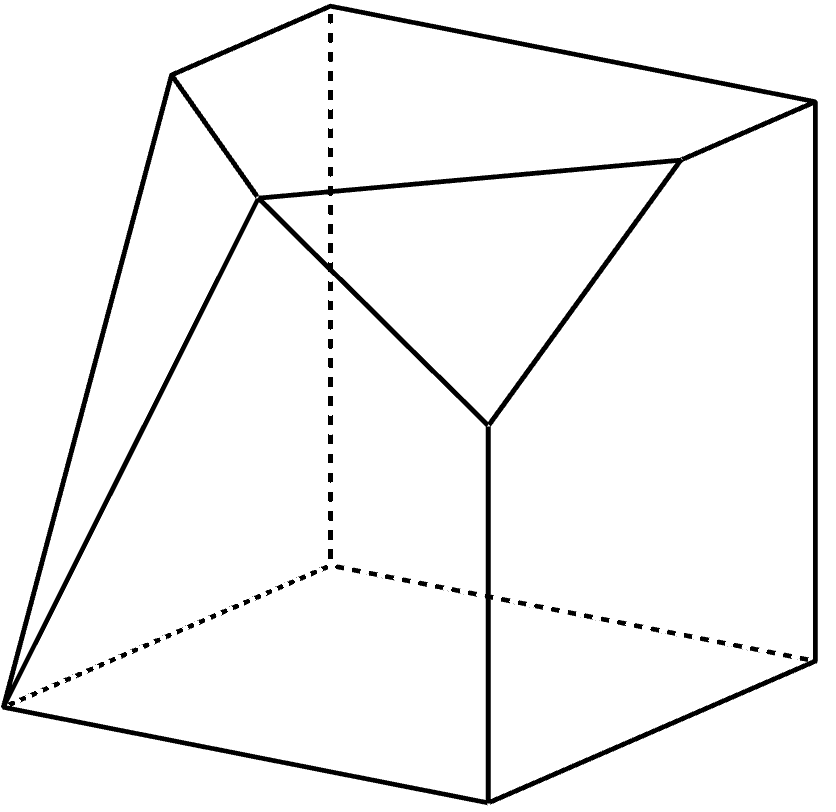
\includegraphics[width=6cm]{poliedro01}
\end{center}
\begin{center}
\begin{tabular}{|c|c|}
\hline 
 & Número \\ 
\hline 
Vértices &  \\ 
\hline 
Faces &  \\ 
\hline 
Arestas &  \\ 
\hline 
\end{tabular} 
\end{center}
\end{multicols}
\end{figure}
\end{problema}

\paragraph{Solução} 

\section{Exercícios}

\begin{enumerate}

\item Complete as tabelas com o número de vértices arestas e faces dos poliedros a seguir:
\begin{enumerate}
\item Primeiro Poliedro

\figura{poliedro01}{5cm}

{
\begin{tabular}{|c|c|}
\hline 
 & Número \\ 
\hline 
Vértices &  \\ 
\hline 
Faces &  \\ 
\hline 
Arestas &  \\ 
\hline 
\end{tabular} 
}

\item Segundo Poliedro

\figura{poliedro02}{5cm}

{
\begin{tabular}{|c|c|}
\hline 
 & Número \\ 
\hline 
Vértices &  \\ 
\hline 
Faces &  \\ 
\hline 
Arestas &  \\ 
\hline 
\end{tabular} 
}

\item Terceiro Poliedro

\figura{poliedro03}{6cm}

{
\begin{tabular}{|c|c|}
\hline 
 & Número \\ 
\hline 
Vértices &  \\ 
\hline 
Faces &  \\ 
\hline 
Arestas &  \\ 
\hline 
\end{tabular} 
}
\end{enumerate}

\item Na figura a seguir é apresentado um tabela com os Sólidos de Platão. Use a fórmula de Euler para preencher s dados que faltam:

\figura{platao}{7cm}

\item O sólido a seguir é um icosaedro truncado, foi usado como formato para a bola da copa do mundo de 1970.

\figura{poliedro04}{5cm}

É um poliedro formado por 12 faces pentagonais regulares e 20 hexagonais regulares. Calcule o número de faces, arestas e vértices do icosaedro truncado.

\item O cubo truncado, figura a seguir, é um poliedro formado pro faces triangulares e octaedrais.
\figura{CuboTruncado}{5cm}

\begin{enumerate}
\item Qual o números de faces triangulares do cubo truncado?
\item Qual o número de arestas do cubo truncado?
\item Qual o número de vértices do cubo truncado?
\end{enumerate}

\item O poliedro a seguir é tetraedro truncado.
\figura{TetraedroTruncado.png}{5cm}

\begin{enumerate}
\item As faces do tetraedro truncado são de dois tipos são polígonos de dois tipos. Quantos e quais são esses polígonos?
\item Quantos são os vértices e arestas do tetraedro truncado?
\end{enumerate}

\item O cuboctaedro é um poliedro formado por 7 faces triangulares e 6 faces quadrangulares, conforme a figura a seguir:
\figura{Cuboctaedro.png}{5cm}

Qual o número de arestas e vértices do Cuboctaedro.

\item O Gran Rombicuboctaedro é um poliedro convexo, no qual suas faces são 6 octaedros, 8 hexágonos e 12 quadriláteros. A seguir é mostrado uma imagem de um Gran Rombicuboctaedro:

\figura{Gran_Rombicuboctaedro.png}{5cm}

Calcule quantas são as arestas do Gran Rombicuboctaedro.

\item O poliedro a seguir é formado por 8 faces triangulares e 6 faces octaedrais.

\figura{poliedro05.png}{5cm}

Calcule o número de vértices e arestas do poliedro anterior:

\item Sabendo que o poliedro a seguir é formado por 10 faces triangulares e 18 faces quadrangulares

\figura{poliedro06.png}{5cm}

Calcule o número de vértices e arestas do poliedro anterior.

\item Calcule o número de faces, vértices e arestas do poliedro a seguir:

\figura{poliedro07.png}{7cm}

\end{enumerate}

\newpage
\begin{center}
\textbf{Questões de\\Múltipla Escolha}
\end{center}

\begin{enumerate}
\item Em um poliedro convexo, o número de arestas excede o número de faces em 18. O número de vértices desse poliedro é:
\begin{enumerate}
\item 10
\item 20
\item 24
\item 30
\item 32
\end{enumerate}

\item  O número de faces triangulares de uma pirâmide é 11. Pode-se, então, afirmar que esta pirâmide possui:
\begin{enumerate}
\item 33 vértices e 22 arestas.
\item 12 vértices e 11 arestas.
\item 22 vértices e 11 arestas.
\item 11 vértices e 22 arestas.
\item 12 vértices e 22 arestas.
\end{enumerate}

\item Sobre as sentenças:

\begin{enumerate}[I.]
\item Um octaedro regular tem 8 faces quadradas.
\item Um dodecaedro regular tem 12 faces pentagonais.
\item Um icosaedro regular tem 20 faces triangulares.
\end{enumerate}
É correto afirmar que apenas:
\begin{enumerate}
\item I é verdadeira.
\item II é verdadeira.
\item III é verdadeira.
\item I e III são verdadeiras.
\item II e III são verdadeiras.
\end{enumerate}

\item Um poliedro convexo tem 12 faces triangulares e as demais, pentagonais. Sabendo que o número de arestas é o triplo do número de faces pentagonais, então a soma dos ângulos de todas as faces pentagonais é, em radianos, igual a:

\begin{enumerate}
\item \m{3\pi}
\item \m{12\pi}
\item \m{36\pi}
\item \m{64\pi}
\item \m{108\pi}
\end{enumerate}

\item  Um poliedro convexo tem seis faces triangulares e cinco faces quadrangulares. O número de arestas e de vértices do poliedro é, respectivamente:
\begin{enumerate}
\item 34 e 10
\item 19 e 10
\item 34 e 20
\item 12 e 10
\item 19 e 12
\end{enumerate}

\item Os sólidos de Platão são poliedros convexos cujas faces são todas congruente a  um único polígono regular, todos os vértices têm o mesmo número de arestas incidentes e cada aresta é compartilhada por apenas duas faces. Eles são importantes, por exemplo, na classificação das formas dos cristais minerais e no desenvolvimento de diversos objetos. Como todo poliedro convexo, os sólidos de Platão respeitam a relação de Euler \m{V-A+F=2}, em que \m{V}, \m{A} e \m{F} são os números de vértices, arestas e faces do poliedro, respectivamente.

Em um cristal, cuja forma é a de um poliedro de Platão de faces triangulares, qual é a relação entre o número de vértices e o número de faces?

\begin{enumerate}
\item \m{2V-4F=4}
\item \m{2V-2F=4}
\item \m{2V-F=4}
\item \m{2V+F=4}
\item \m{2V+5F=4}
\end{enumerate}

\item O número de vértices de um poliedro convexo que possui 12 faces, todas triangulares é:
\begin{enumerate}
\item 4
\item 12
\item 10
\item 6
\item 8 
\end{enumerate}

\item O hábito cristalino é um termo utilizado por mineralogistas para descrever a aparência típica de um cristal em termos de tamanho e forma. A granada é um mineral cujo hábito cristalino é um poliedro com 30 arestas e 20 vértices. Um mineralogista construiu um modelo ilustrativo de um cristal de granada pela junção dos polígonos correspondentes às faces. Supondo que o poliedro ilustrativo de um cristal de granada é convexo, então a quantidade de faces utilizadas na montagem do modelo ilustrativo desse cristal é igual a
\begin{enumerate}
\item 10
\item 12
\item 25
\item 42
\item 50
\end{enumerate}

\item Um geólogo encontrou, numa de suas explorações, um cristal de rocha no formato de um poliedro, que satisfaz a relação de Euler, de 60 faces triangulares. O número de vértices deste cristal é iguala:
\begin{enumerate}
\item 35
\item 34
\item 33
\item 32
\item 31
\end{enumerate}


\item Em um poliedro convexo, o número de arestas excede o número de faces em 18. O número de vértices desse poliedro é:
\begin{enumerate}
\item 10
\item 20
\item 24
\item 30
\item 32
\end{enumerate}

\item O número de faces triangulares de uma pirâmide é 11. Pode-se, então, afirmar que esta pirâmide possui:
\begin{enumerate}
\item 33 vértices e 22 arestas.
\item 12 vértices e 11 arestas.
\item 22 vértices e 11 arestas.
\item 11 vértices e 22 arestas.
\item 12 vértices e 22 arestas.
\end{enumerate}

\item  Sobre as sentenças:
\begin{enumerate}[I.]
\item Um octaedro regular tem 8 faces quadradas.
\item Um dodecaedro regular tem 12 faces pentagonais.
\item Um icosaedro regular tem 20 faces triangulares.
\end{enumerate}

É correto afirmar que apenas:
\begin{enumerate}
\item I é verdadeira.
\item II é verdadeira.
\item III é verdadeira.
\item I e III são verdadeiras.
\item II e III são verdadeiras.
\end{enumerate}

\item  Um poliedro convexo tem seis faces triangulares e cinco faces quadrangulares. O número de arestas e de vértices do poliedro é, respectivamente:
\begin{enumerate}
\item 34 e 10
\item 19 e 10
\item 34 e 20
\item 12 e 10
\item 19 e 12
\end{enumerate}
\end{enumerate}


\begin{exercicio}

\begin{figure}[!htb]
\center
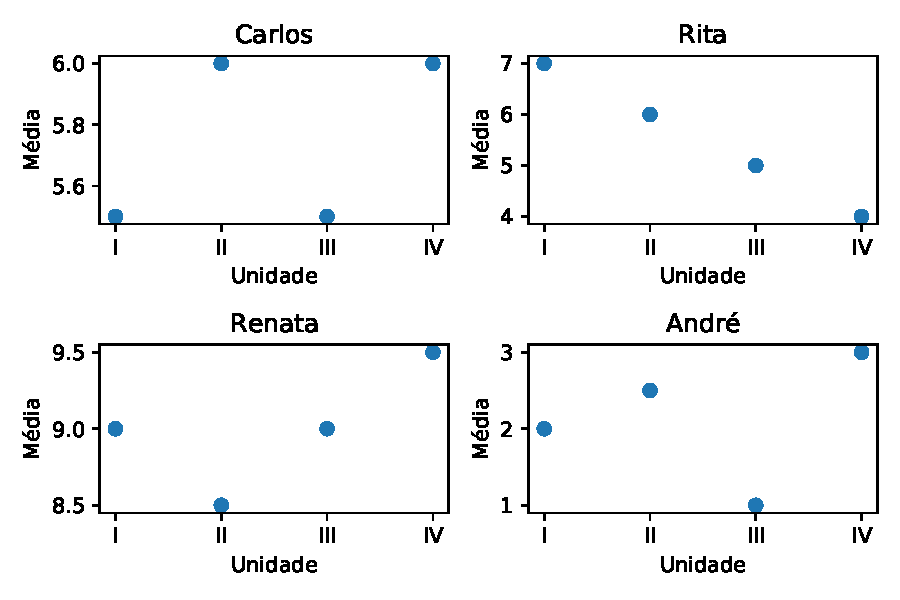
\includegraphics[width=10cm]{01}
\end{figure}

\end{exercicio}

\section{Atividade}
\begin{enumerate}
\item Completando as tabelas com o número de vértices arestas e faces dos poliedros a seguir, qual o número de arestas do poliedro:
\begin{figure}[!htb]
\begin{multicols}{2}
\begin{center}
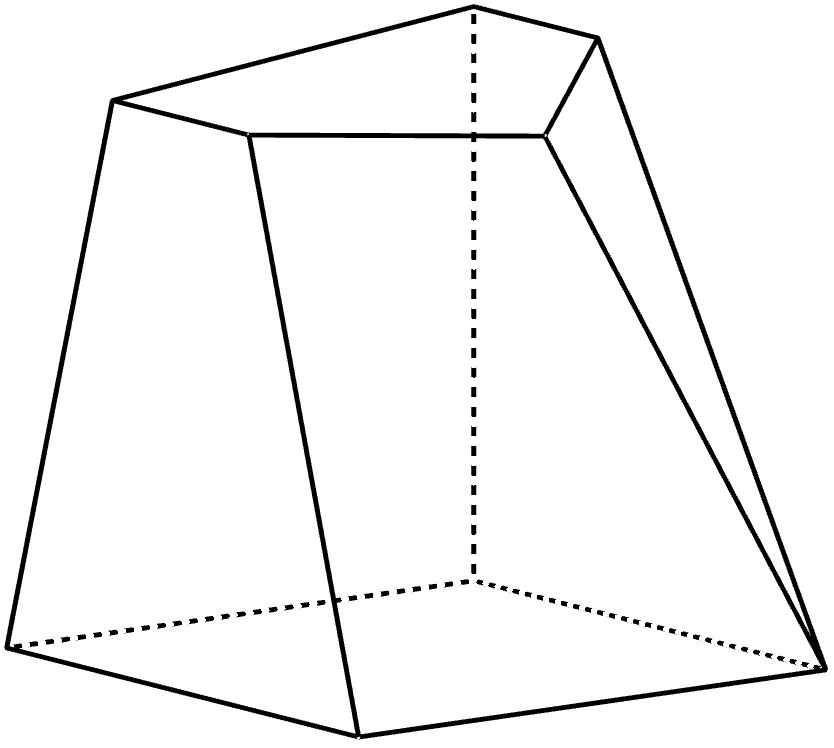
\includegraphics[width=6cm]{poliedro02}
\end{center}
\begin{center}
\begin{tabular}{|c|c|}
\hline 
 & Número \\ 
\hline 
Vértices &  \\ 
\hline 
Faces &  \\ 
\hline 
Arestas &  \\ 
\hline 
\end{tabular} 
\end{center}
\end{multicols}
\end{figure}
\end{enumerate}

\end{document}